\let\negmedspace\undefined
\let\negthickspace\undefined
\documentclass[journal]{IEEEtran}
\usepackage[a5paper, margin=10mm, onecolumn]{geometry}
%\usepackage{lmodern} % Ensure lmodern is loaded for pdflatex
\usepackage{tfrupee} % Include tfrupee package

\setlength{\headheight}{1cm} % Set the height of the header box
\setlength{\headsep}{0mm}     % Set the distance between the header box and the top of the text

\usepackage{gvv-book}
\usepackage{gvv}
\usepackage{cite}
\usepackage{amsmath,amssymb,amsfonts,amsthm}
\usepackage{algorithmic}
\usepackage{graphicx}
\usepackage{textcomp}
\usepackage{xcolor}
\usepackage{txfonts}
\usepackage{listings}
\usepackage{enumitem}
\usepackage{mathtools}
\usepackage{gensymb}
\usepackage{comment}
\usepackage[breaklinks=true]{hyperref}
\usepackage{tkz-euclide} 
\usepackage{listings}
% \usepackage{gvv}                                        
\def\inputGnumericTable{}                                 
\usepackage[latin1]{inputenc}                                
\usepackage{color}                                            
\usepackage{array}                                            
\usepackage{longtable}                                       
\usepackage{calc}                                             
\usepackage{multirow}                                         
\usepackage{hhline}                                           
\usepackage{ifthen}                                           
\usepackage{lscape}
\begin{document}

\bibliographystyle{IEEEtran}
\vspace{3cm}


\title{1-1.4-11}
\author{EE24BTECH11004 - ANKIT JAINAR
}
% \maketitle
% \newpage
% \bigskip
{\let\newpage\relax\maketitle}

\renewcommand{\thefigure}{\theenumi}
\renewcommand{\thetable}{\theenumi}
\setlength{\intextsep}{10pt} % Space between text and floats


\numberwithin{equation}{enumi}
\numberwithin{figure}{enumi}
\renewcommand{\thetable}{\theenumi}

\textbf{Question:} Find the coordinates of the points which divide the line segment joining A(-2, 2) and B(2, 8) into four equal parts.\\
\solution:Using the section formula for internal division, the coordinates of the point dividing the line in the ratio $k:1$ are given by:

\begin{align}
R_k &= \left( \frac{x_2  + k \cdot x_1}{k+1}, \frac{ y_2 + k \cdot y_1}{k+1} \right)
\end{align} 
where $k = \frac{i}{n-i}$ $n$, $0<i<n$ is number of equal parts \\
For $n = 4$ \\
now for
\begin{align}
R_1,k&=\frac{1}{3}\\
R_2,k&=1\\
R_3,k&=3\\
\end{align}
by substituting A=\brak{-2,2} and B=\brak{2,8} in $R_k$
we get \\
\begin{align}
   R_1&=\brak{-1.0,3.5}\\
   R_2&=\brak{0.0,5.0}\\
   R_3&=\brak{1.0,6.5}\\
\end{align}	

\begin{figure}
    \centering
    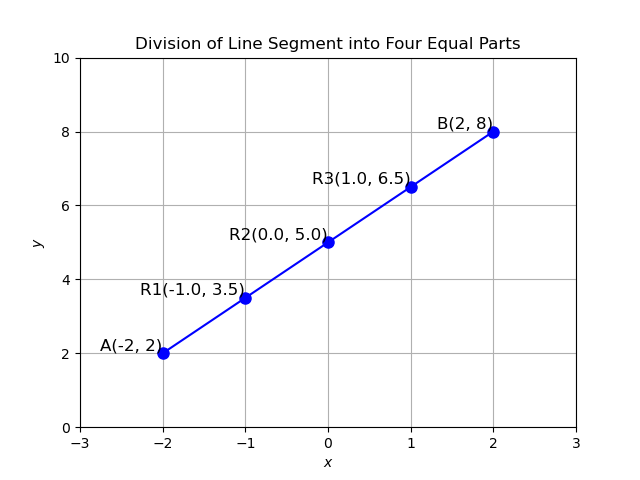
\includegraphics[width=0.5\linewidth]{figs/Figure_1.png}
    \caption{Stem Plot of y\brak{n}}
    \label{stemplot}
\end{figure}



\end{document}
